\chapter{Tensor networks (TN)}
\label{ch:tn}

Quantum many-body systems are naturally represented in spaces of high-rank tensors, and the demand to decompose them into smaller tensors has arisen in studies of their entanglement properties~\cite{white1992density}. The diagrammatic notations of tensors, namely Penrose graphical notations~\cite{penrose1971applications}, have greatly eased the construction and reasoning of complicated contractions with multiple tensors, known as tensor networks (TN)~\cite{bridgeman2017hand, orus2014practical}. Their use has been widely promoted in various fields of physics besides condensed matters, including quantum computing~\cite{feynman1986quantum, nielsen2010quantum}, high-energy physics~\cite{banuls2018tensor, banuls2020review}, and quantum gravity~\cite{perez2013spin, you2016entanglement, hayden2016holographic, asaduzzaman2020tensor}.

TNs can also be used as variational ansatzes, which enable exact and efficient summation over exponentially many configurations, instead of Monte Carlo sampling. Compared to neural networks, TNs are usually more controllable and systematically improvable, in the sense that they have few hyperparameters prone to manual tuning, and by tuning these hyperparameters, we can continuously improve the accuracy of variational approximation at the cost of more computation, which may allow extrapolating the variational results to the limit of infinite expressiveness.

\begin{figure}[htb]
\centering
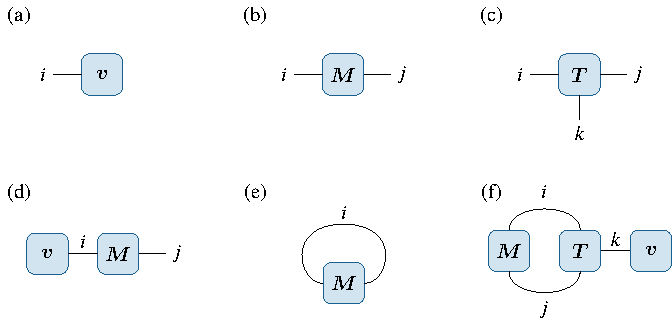
\includegraphics[width=0.7\linewidth]{ch8/tensors.pdf}
\caption[Tensor diagram notations]{
Examples of tensor diagram notations.
(a) A vector $\vv$ with an index $i$.
(b) A matrix $\mM$ with two indices $i, j$.
(c) A tensor $\mT$ with three indices $i, j, k$.
(d) The matrix-vector multiplication $\sum_i v_i M_{i j}$, where $j$ is left as a free index.
(e) The matrix trace $\sum_i M_{i i}$.
(f) The tensor contraction $\sum_{i, j, k} T_{i j k} M_{i j} v_k$.
}
\label{fig:tensors}
\end{figure}

\section{Tensor diagram notations}

For the purpose of this thesis, we think of tensors as multidimensional arrays, and we do not emphasize their invariance under symmetry operations. In the diagrammatic notations, each tensor is a node in the diagram, and its indices are denoted by ``legs'' stretching out from the node\footnote{Some literature distinguishes between covariant and contravariant indices, but we do not distinguish between them in this thesis, and we allow contracting any two indices as long as they are defined in the same space.}. The contraction between two indices is denoted by connecting the two legs. Some examples of tensor diagrams are shown in \cref{fig:tensors}.

In principle, when the tensor is not symmetric in any two indices, we need to specify which of its legs corresponds to which index, e.g., whether \cref{fig:tensors}~(f) represents $\sum_{i, j, k} T_{i j k} M_{i j} v_k$ or $\sum_{i, j, k} T_{i j k} M_{j i} v_k$. But we usually omit this specification for brevity when it can be inferred from the context. Also, we omit the names of indices when not needed.

\section{Matrix product state (MPS)}

\begin{figure}[htb]
\centering
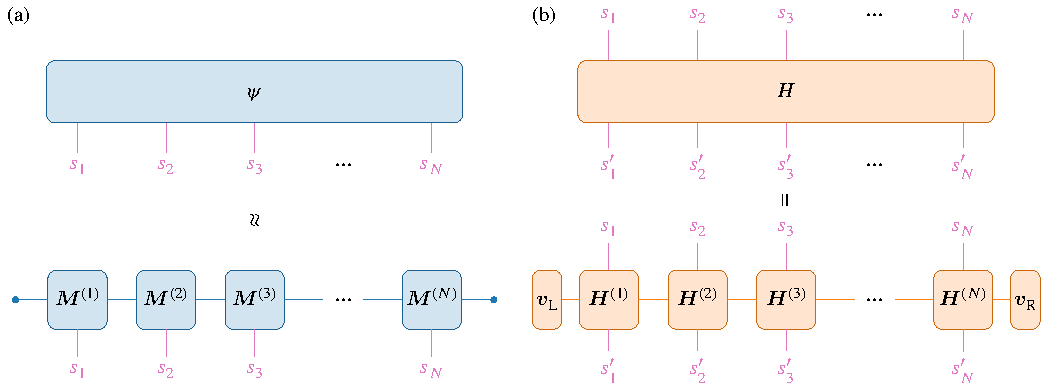
\includegraphics[width=\linewidth]{ch8/mps_mpo.pdf}
\caption[Matrix product state (MPS) and matrix product operator (MPO)]{
(a) A quantum many-body wave function $\psi(s_1, \ldots, s_N)$ approximated by a matrix product state (MPS).
The {\color[HTML]{e377c2} pink} legs can take spin values, the {\color[HTML]{1f77b4} blue} legs have the MPS bond dimension $\chi$, and the solid dot denotes summing over an index. \\
(b) A Hamiltonian $H(s_1, \ldots, s_N; s'_1, \ldots, s'_N)$ represented by a matrix product operator (MPO).
The {\color[HTML]{ff7f0e} orange} legs have the MPO bond dimension $\chi_H$.
}
\label{fig:mps-mpo}
\end{figure}

For a quantum many-body system of $N$ spin-$\frac{1}{2}$ particles, the wave function $\psi(\vs)$ lives in a Hilbert space of $2^N$ dimensions, as defined in \cref{sec:qu-sys}. We can view $\psi(\vs)$ as a tensor with $N$ indices $s_1, s_2, \ldots, s_N$, and each index can take the spin values, which we denote by $\{\spinup, \spindown\}$, and also represented as $\{0, 1\}$ when using $0$-based numeric array indexing. This tensor is visualized at the top of \cref{fig:mps-mpo}~(a).

The matrix product state (MPS) is a TN ansatz to approximately decompose $\psi(\vs)$ into a product of rank-$3$ tensors\footnote{Although they are rank-$3$ tensors, for historical reasons the ansatz is still named ``matrix'' product state.}, also known as the tensor train decomposition~\cite{oseledets2011tensor}. It is formally defined by
\begin{equation}
\psi(\vs) = \sum_{a_0, \ldots, a_N = 1}^\chi \prod_{i = 1}^N M^{(i)}_{s_i; a_i, a_{i - 1}},
\label{eq:mps}
\end{equation}
and visualized at the bottom of \cref{fig:mps-mpo}~(a). Here $\chi$ is called the bond dimension, which is the most important hyperparameter of the MPS to control its overall size and expressiveness, and each bond index $a_i$ runs in $1, \ldots, \chi$. Different sites can have different $\chi$, as we will discuss in \cref{sec:dmrg}, but we simply use a typical value of $\chi$ when analyzing the computational complexity of MPS. Therefore, the MPS contains $2 N \chi^2$ variational parameters, which is an exponential reduction from the $2^N$ dimensional Hilbert space.

Note that we have imposed the open boundary conditions (OBC) in the MPS, where the indices $a_0$ and $a_N$ at the two ends are simply summed over, which are equivalent to contracting with two vectors of ones, denoted by the solid dots in \cref{fig:mps-mpo}. These summations also make some parameters in $\mM^{(1)}$ and $\mM^{(N)}$ redundant. The OBC and the finite system size rule out the translational symmetry, so we do not share parameters $\mM^{(i)}$ between different sites $i$. There are also methods to study the limit of infinite system size, where $\mM^{(i)}$ obeys the translational symmetry~\cite{mcculloch2008infinite}.

\section{Contraction of MPS}
\label{sec:mps-contract}

\begin{figure}[htb]
\centering
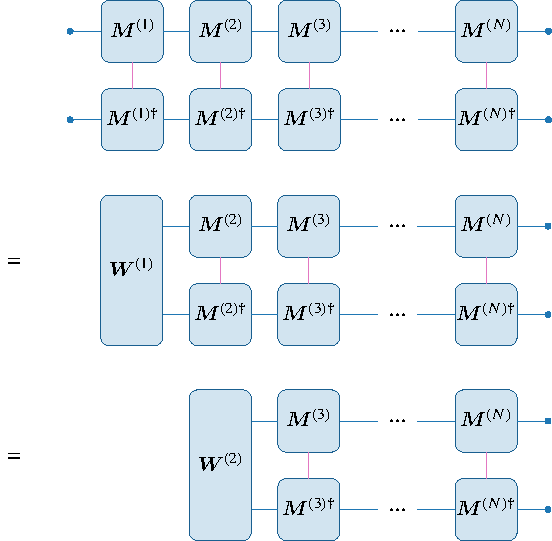
\includegraphics[width=0.6\linewidth]{ch8/mps_contract.pdf} \hspace{2cm}
\caption[Sequential contraction of MPS]{
Sequential contraction of an MPS and its conjugate, where $\mW^{(i)}$ is the intermediate result after the $i$-th step. In each step, we contract $\mW^{(i - 1)}$ and $\mM^{(i)}$, then contract the result with $\mM^{(i) \dagger}$ to obtain $\mW^{(i)}$, which takes $O(\chi^3)$ time and $O(\chi^2)$ space.
}
\label{fig:mps-contract}
\end{figure}

Besides the parameter efficiency, another advantage of MPS is that we can exactly and efficiently compute the normalization constant $\ip{\psi}$ by contracting the MPS with the conjugate of itself. As shown in \cref{fig:mps-contract}, this contraction is performed site-by-site. In each step, we contract the intermediate result $\mW^{(i - 1)}$ and a tensor $\mM^{(i)}$ to obtain
\begin{equation}
V^{(i)}_{s; a_i, a'_{i - 1}} = \sum_{a_{i - 1}} M^{(i)}_{s; a_i, a_{i - 1}} W^{(i - 1)}_{a_{i - 1}, a'_{i - 1}},
\end{equation}
which takes $O(\chi^3)$ time. Then we contract $\mV^{(i)}$ and $\mM^{(i) \dagger}$ to obtain
\begin{equation}
W^{(i)}_{a_i, a'_i} = \sum_{s, a'_{i - 1}} M^{(i) \dagger}_{s; a'_i, a'_{i - 1}} V^{(i)}_{s; a_i, a'_{i - 1}},
\end{equation}
which also takes $O(\chi^3)$ time. Therefore, the contraction of $N$ sites takes $O(N \chi^3)$ time, which is also an exponential reduction from naively summing over the $2^N$ configurations. In addition, we can see that if we impose periodic boundary conditions (PBC) rather than OBC, i.e., connect the solid dots at the two ends of the MPS, then the intermediate result $\mW^{(i - 1)}$ has to maintain four indices of size $\chi$, therefore the time complexity to contract the above TN increases to $O(N \chi^4)$, while the dynamic space required by the intermediate result increases even more rapidly from $O(\chi^2)$ to $O(\chi^4)$.

\section{Matrix product operator (MPO)}
\label{sec:mpo}

When using MPS to study the ground state of a Hamiltonian, we need to decompose the latter into a similar form as the former, namely matrix product operator (MPO), as visualized in \cref{fig:mps-mpo}~(b). The MPO also has a bond dimension $\chi_H$, and we usually set $\chi \gg \chi_H$ in large-scale computations. Unlike MPS, the boundary conditions of MPO are not simply imposed by summing over the indices, but contracting with specific vectors depending on the Hamiltonian, as denoted by $\vv_\text{L}$ and $\vv_\text{R}$ in \cref{fig:mps-mpo}~(b).

In the same manner discussed in \cref{sec:mps-contract}, the expectation of the Hamiltonian $\mel{\psi}{\hat{H}}{\psi}$ without the normalization can be exactly contracted in $O(\chi^3)$ time and $O(\chi^2)$ space. Other observable besides the Hamiltonian can also be measured in this manner, which is especially efficient if the operator only acts on one or few sites.

Algorithms have been proposed to exactly or approximately construct an MPO from a locally interacting operator~\cite{crosswhite2008finite, hubig2017generic, paeckel2017automated}. As a concrete example, the MPO exactly equivalent to the Hamiltonian of the transverse field Ising model in \cref{eq:qu-ising} is given by
\begin{align}
\mH^{(i)} &= \begin{pmatrix}
\hat{I} & 0 & 0 \\
\hat{\sigma}^z & 0 & 0 \\
\Gamma \hat{\sigma}^x & J \hat{\sigma}^z & \hat{I}
\end{pmatrix}, \\
\vv_\text{L} &= \begin{pmatrix} 0 & 0 & \hat{I} \end{pmatrix}, \\
\vv_\text{R} &= \begin{pmatrix} \hat{I} & 0 & 0 \end{pmatrix}^\transpose,
\end{align}
where the matrix and the vectors have bond indices, while the operators have spin indices. Substitute this definition into \cref{fig:mps-mpo}~(b) and contract the TN, the original Hamiltonian will be recovered.

Before modern numerical approaches were possible, MPS with small $\chi$ has been successfully applied in the analytical solutions to the ground states of many one-dimensional systems, including the renowned Affleck--Kennedy--Lieb--Tasaki (AKLT) model of the spin-$1$ Heisenberg chain~\cite{affleck1987rigorous, klumper1991equivalence, fannes1992finitely}, and the Majumdar--Gosh model with the addition of next-nearest-neighbor frustrated interaction~\cite{majumdar1969next}. It has been proven that if we cut an MPS into two parts, then the entanglement entropy $S$ between them scales at most by $S = O(\ln \chi)$, therefore MPS is suitable for representing states with low entanglement\cite{verstraete2008matrix}. Moreover, the spatial correlation of any single-site operator
\begin{equation}
C(d) = \frac{1}{N - d} \sum_{i = 1}^{N - d} \ev{\hat{O}_i \hat{O}_{i + d}} - \ev{\hat{O}_i} \ev{\hat{O}_{i + d}}
\label{eq:corr-d}
\end{equation}
decays exponentially: $C(d) \sim \rme^{-\frac{d}{\xi}}$, where $\xi$ is the correlation length. This is exactly the case for the ground states of 1D gapped systems, so it is possible for MPS to exactly represent them.

\section{Density matrix renormalization group (DMRG)}
\label{sec:dmrg}

\begin{figure}[htb]
\centering
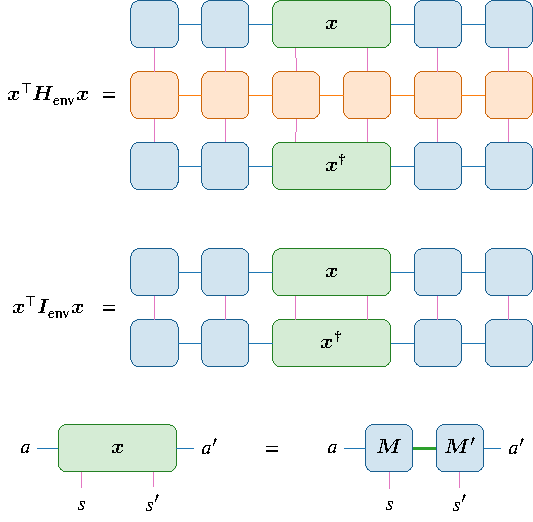
\includegraphics[width=0.7\linewidth]{ch8/dmrg.pdf}
\caption[Density matrix renormalization group (DMRG)]{
Tensor diagrams used in the density matrix renormalization group (DMRG) algorithm. We show six sites as an example, and omit the vectors on the boundaries for clarity. \\
(a) Obtaining the environment tensor $\mH_\text{env}$ by contracting $\mel{\psi}{\hat{H}}{\psi}$ apart from the two sites $\vx$ to be updated. \\
(b) Obtaining the environment tensor $\mI_\text{env}$ by contracting $\ip{\psi}$ apart from $\vx$. \\
(c) Decomposing the updated $\vx$ into two sites, where the thick green index $b$ can have a dimension $\chi'$ different from the original $\chi$.
}
\label{fig:dmrg}
\end{figure}

Along with the analytical studies, the numerical approach to optimize MPS for variational ground state approach developed at the same time. As the name suggests, the density matrix renormalization group (DMRG) algorithm~\cite{white1992density, schollwock2005density} originated from the theory of renormalization group, but for the purpose of this thesis we can simply think of it as an iterative series of two-site updates.

In each step, we choose a site $\mM^{(i)}$ and its neighbor $\mM^{(i + 1)}$, and contract $\mel{\psi}{\hat{H}}{\psi}$ and $\ip{\psi}$ respectively, apart from the two sites to be updated, and obtain the environment tensors $\mH_\text{env}$ and $\mI_\text{env}$, as shown in \cref{fig:dmrg}~(a) and (b). Then we view $\mel{\psi}{\hat{H}}{\psi}$ and $\ip{\psi}$ as $4 \chi^2 \times 4 \chi^2$ matrices, and solve the optimization problem
\begin{equation}
\arg\min_\vx \frac{\vx^\dagger \mH_\text{env} \vx}{\vx^\dagger \mI_\text{env} \vx},
\end{equation}
which is equivalent to the generalized eigenvector problem
\begin{equation}
\mH_\text{env} \vx = \lambda \mI_\text{env} \vx
\end{equation}
with the smallest eigenvalue $\lambda$, and can be solved in $O(\chi^4)$ time and space.

After obtaining $\vx$, it needs to be decomposed into the updated sites $\mM^{(i)}$ and $\mM^{(i + 1)}$, as shown in \cref{fig:dmrg}~(c). We can view $\vx$ as a $2 \chi \times 2 \chi$ matrix, whose rank is at most $2 \chi$, so in general the dimension of the index $b$ after the decomposition can also be $2 \chi$. If we want $\mM^{(i)}$ and $\mM^{(i + 1)}$ to have the same size as before, we can use singular value decomposition (SVD) to obtain the best approximation of them, where we only keep the first $\chi$ singular values. Alternatively, we can control the new bond dimension $\chi'$ between $\mM^{(i)}$ and $\mM^{(i + 1)}$ by discarding the singular values below a threshold, therefore the size of the ansatz is dynamically adapted during the DMRG procedure, which depends on the amount of entanglement in the physical system.

The above step of DMRG can only update parameters of two sites. We usually apply $N - 1$ steps on all sites sequentially, and call it a ``sweep''. After sufficiently many sweeps, the parameters of all sites will converge to the best approximation. This algorithm is also known as alternating least square (ALS) in other fields of optimization problems~\cite{comon2009tensor, dolgov2015corrected}. As a second-order optimization algorithm, it can have faster convergence speed than the gradient descent (GD) optimizer, and avoid some local minima and saddle points that the latter is prone to. The extensions to second-order optimizers discussed in \cref{sec:ngd} can also be applied to DMRG, including the damping to improve stability and the low-rank updates to reduce memory usage.

It is worth noting that the above MPS also supports evaluating $\psi(\vs)$ given a configuration $\vs$, i.e., specifying a spin value at each spin index and contracting the remaining TN, which takes $O(\chi^3)$ time and $O(\chi^2)$ space. In principle, MPS can be optimized by GD in the framework of VMC, instead of DMRG, especially when PBC is imposed and the computational complexity of DMRG is polynomially higher~\cite{sandvik2007variational}. The gradients through tensor contractions and SVD truncations can be obtained by automatic differentiation~\cite{liu2017gradient, liao2019differentiable}. Moreover, MPS supports exact sampling in the autoregressive form~\cite{ferris2012perfect, han2018unsupervised, wei2022sequential}, which we will discuss in more depth in \cref{ch:tensor-rnn}.

Besides DMRG, another optimization algorithm arisen from the physical properties of MPS is the time-evolving block decimation (TEBD) algorithm~\cite{vidal2003efficient}, which decomposes the Hamiltonian into one- or two-site blocks and apply them to the MPS sequentially. It can be more efficient than DMRG for systems with PBC or higher-dimensional geometries, as it avoids contracting the environment tensors~\cite{jiang2008accurate}.

\section{TN with higher-dimensional geometries}

In the previous sections, we have seen that MPS can be analytical or numerically exact solutions to the ground states of many 1D systems, and it only requires polynomial time and space to exactly evaluate observables. However, it is no longer so efficient for systems on 2D or higher-dimensional geometries.

The applicability of MPS can be examined by the area law of entanglement entropy~\cite{srednicki1993entropy, verstraete2006criticality, hastings2007area, eisert2010colloquium}: For gapped and locally interacting systems, when we cut out a region from it, the entanglement entropy $S$ between the region and the environment is asymptotically proportional to the area of the boundary, rather than the volume of the region. For 1D systems, the boundary consists of only two sites, so we have $S = O(1)$, which can be captured by an MPS if its bond dimension $\chi$ is large enough.

For a 2D system with $N$ sites, we have $S = O(L)$, where $L = O(N^\frac{1}{2})$ is the linear size of the system. When applying an MPS to it, we need to arrange it in an 1D order of the sites, and some possible choices are sketched in \cref{fig:mps-order}. Regardless of how we choose the order, we can always cut the MPS into two parts, i.e., divide the system into $\vs_{\le k} = \{s_i \mid 1 \le i \le k\}$ and $\vs_{> k} = \{s_i \mid k < i \le N\}$, where the index $i$ follows the order of the MPS, and the bond between the sites $k$ and $k + 1$ is cut. Therefore, the entanglement entropy between $\vs_{\le k}$ and $\vs_{> k}$ produced by the MPS is $S = O(\ln \chi)$, and we can obtain the expected area law only if the bond dimension $\chi = O(\rme^L)$, which is considered intractable when $L$ is large.

\begin{figure}[htb]
\centering
\hspace*{\fill}
\subfloat[]{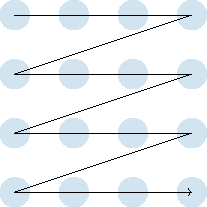
\includegraphics[width=0.2\linewidth]{ch8/mps_order_zigzag.pdf}}
\hspace*{\fill}
\subfloat[]{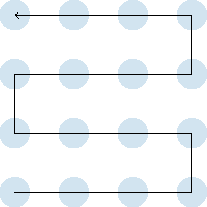
\includegraphics[width=0.2\linewidth]{ch8/mps_order_snake.pdf}}
\hspace*{\fill}
\subfloat[]{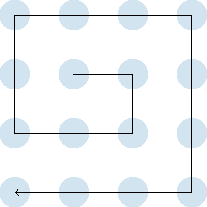
\includegraphics[width=0.2\linewidth]{ch8/mps_order_spiral.pdf}}
\hspace*{\fill}
\subfloat[]{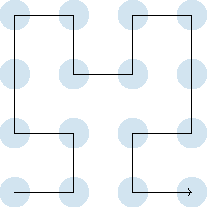
\includegraphics[width=0.2\linewidth]{ch8/mps_order_hilbert.pdf}}
\hspace*{\fill}
\caption[Orders of MPS on 2D lattice]{
Different orders of MPS on 2D lattices, where a $4 \times 4$ lattice is shown as an example: (a) zigzag order, (b) snake order, (c) spiral order, (d) Hilbert space-filling curve~\cite{hilbert1891uber}.
}
\label{fig:mps-order}
\end{figure}

The lack of entanglement in MPS is also shown in the correlations of observables. The correlations in MPS decay by $C(d) \sim \rme^{-\frac{d}{\xi}}$, where $r$ is the distance in the 1D order. However, the 1D order breaks the locality of the 2D distance. For example, when we use the zigzag order as in \cref{fig:mps-order}~(a), every pair of vertically adjacent sites have spatial distance $1$, but their distance in the 1D order is as large as $L$, which makes it difficult for the MPS to capture their correlation. One may attempt to arrange the MPS in a more complicated order with better locality, such as the Hilbert space-filling curve~\cite{hilbert1891uber} in \cref{fig:mps-order}~(d), but it has been proven that no 1D order is substantially better than the most naive zigzag order for preserving the distances of all pairs of sites on the 2D lattice~\cite{xu2012lower}.

These difficulties motivate us to propose ansatzes with 2D geometries natively for 2D systems, and a relatively simple and prevalent choice is the projected entangled-pair state (PEPS)~\cite{verstraete2004renormalization, verstraete2008matrix}. While it originated from the representation of two-site entanglements, in the context of variational ansatzes it usually refers to the most intuitive generalization of MPS to 2D, as shown in \cref{fig:peps}.

\begin{figure}[htb]
\centering
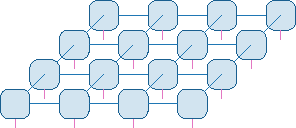
\includegraphics[width=0.6\linewidth]{ch8/peps.pdf}
\caption[Projected entangled-pair state (PEPS)]{
Projected entangled-pair state (PEPS) as the generalization of MPS to 2D, on a $4 \times 4$ lattice as an example.
A tensor of size $2 \times \chi \times \chi \times \chi \times \chi$ is placed on each site.
The vectors on the boundaries are omitted for clarity.
}
\label{fig:peps}
\end{figure}

When we cut out a region from a PEPS, there are always $O(L)$ bonds across the boundary, and we can view the whole boundary as a thick bond of size $\chi^{O(L)}$. Therefore, the entanglement entropy produced by the MPS is $S = O(L \ln \chi)$, which can achieve the area law. It has also been shown by construction that PEPS can exactly represent some states with the area law, such as the resonating valence bond (RVB) state~\cite{schuch2012resonating} to describe spin liquids, and the Toric code~\cite{kitaev2003fault, schuch2010peps} useful in quantum computing. Moreover, PEPS can produce algebraically\footnote{Here ``algebraic'' means decaying in a power law, as opposed to exponentially decaying.} decaying correlations~\cite{verstraete2006criticality}, which is a property of 2D critical systems.

However, the main drawback of PEPS is that we cannot exactly contract $\ip{\psi}$ or evaluate $\psi(\vs)$ in polynomial time and space. It is impossible to sequentially contract a PEPS and keep a fixed number of free indices in the intermediate result, as in \cref{fig:mps-contract}, while a growing number of free indices leads to exponentially growing time and space complexities. It has been proven that contracting a general PEPS belongs to the \#P-hard class of computational complexity~\cite{schuch2007computational}, which is considered intractable for large systems.

A practical approach is to approximately contract the PEPS and use SVD to truncate the intermediate result, such that the time and the space complexities remain polynomial. When optimizing a PEPS using DMRG, the environment tensors can be contracted in this approach, which has been successfully applied to systems with more than $1000$ spins~\cite{stoudenmire2012annual, lubasch2014algorithms, vanderstraeten2022variational}. Besides regular lattices, this approach can also contract more complicated TNs on unstructured graphs~\cite{jermyn2020automatic, pan2020contracting, sahu2022efficient}, which is useful in disordered systems with random interactions, as well as quantum circuits. Alternatively, TNs contracted in this approach can be optimized by GD in the framework of VMC~\cite{schuch2008simulation, mezzacapo2009ground, vanderstraeten2016gradient}.

The difficulty of contracting PEPS is caused by the loops in the 2D grid, and other TNs with loop-free and tree-like architectures have been proposed~\cite{shi2006classical, silvi2010homogeneous, cheng2019tree, felser2021efficient}. Some of them can be exactly contracted, at the cost of reduced expressiveness. A renowned architecture is the multiscale entanglement renormalization ansatz (MERA)~\cite{vidal2007entanglement, qian2022tree}, which can produce algebraically decaying correlations, but not the 2D area law, in polynomial computation time and space. Numerically, they have been optimized to higher accuracies than MPS ever achieved on 2D systems.
